\documentclass{article}
\usepackage{ifthen}
\usepackage{color}
\usepackage{tikz}
\usetikzlibrary{trees}
\usepackage{bussproofs}
\EnableBpAbbreviations



\usepackage[paper=a4paper,margin=1in]{geometry}
\usepackage{array}
\usepackage{listings}
\def\lstxml{
  \lstset{language=XML,
    keywordstyle=\ttfamily,
    identifierstyle=\ttfamily,
    stringstyle=\ttfamily,
    showstringspaces=false,
    columns=[l]flexible,
    escapeinside={(@*}{*@)},
    morekeywords={encoding,
      mrow,math,mfrac,mi,msqrt,mo,mn,span,nobr,img}
  }
}
\def\depr#1{#1 (\textit{Deprecated?})}
\def\mathml#1{\texttt{#1}}


\title{Speech Rule Engine:\\ Semantic Tree Grammar}
\author{Volker Sorge}

\begin{document}
\maketitle

Sections~\ref{sec:types},~\ref{sec:roles},~\ref{sec:fonts} presents the types,
roles and fonts used in the semantic representation. Types are used as tags in
corresponding XML representation, while roles and fonts are attributes.

\section{Types}
\label{sec:types}

Types are immutable. Their idea is to capture the basic natur of a symbol.

\subsection{Primitive Types}
\label{sec:primitive types}

They are assigned by default to single symbols (or combination in the case of
numbers, functions, units) and never change.

\begin{tabular}{>{\tt}ll}
  punctuation & Punctuation like comma, dot, ellipses.\\
  fence & Fence symbol.\\
  number & One or several digits, plus some punctuation.\\
  identifier & Single or multiple letters.\\
  text & Regular text in a math expression.\\
  operator & e.g. $+, *$.\\
  relation & Relation symbol, e.g. equals.\\
  largeop & e.g. Sum, product, integral.\\
  function & Some named function.\\
\end{tabular}

\subsection{Compound Types}
\label{sec:compound types}

They are computed once and then never change.


\begin{tabular}{>{\tt}ll}
\multicolumn{2}{l}{\textbf{Compound Symbols}}\\
accent & \depr{Accented symbols}\\
fenced & Fenced expression\\
fraction & Fractions \\
punctuated & List of punctuated elements\\
\multicolumn{2}{l}{\textbf{Relations}}\\
relseq & Relation sequence of a single relation.\\
multirel & Relation sequence containing at least two different relations.\\
\multicolumn{2}{l}{\textbf{Operations}}\\
infixop & Infix operator like $+,\cdot$.\\
prefixop & Prefix operator like $f(x), \sin(x)$ etc.\\
postfixop & Postfix operator like \texttt{x++, y--}\\
\end{tabular}

\begin{tabular}{>{\tt}lp{13cm}}
  \multicolumn{2}{l}{\textbf{Function and big operator applications}}\\
  appl & General function application\\
  integral & Integral expression\\
  bigop & Big operator expression such as a sum or product.\\
  sqrt & Square root expression, i.e., surds without argument or argument $=2$\\
  root & Root expression, i.e., surds with argument $\not=2$ \\
  \multicolumn{2}{l}{\textbf{Big operators or functions with limits or indices}}\\
  limupper & Large operators or limit functions with upper limit expressions. 
             Note the difference to the \textit{script} and \textit{score} types.\\
  limlower & Large operators or limit functions with lower limit. \\
  limboth & Large operators or limit functions with upper and lower limit. \\
  subscript & Subscript expression; can have role subsup, meaning that it originated from an msubsup.\\
  superscript & Superscript expression.\\
  underscore & Stacked expression with underscript.\\
  overscore & Stacked expression with overscript.\\
  tensor & Tensor with four indices. At least one left index is present otherwise it
           would be sub-superscript expression. \\

  \multicolumn{2}{l}{\textbf{Tables and their elements}}\\
  table & A layout element with multiple columns and one or multipled rows. It contains rows and cells.\\
  multiline & A layout element with one or multiple rows, where each row contains at
              most one element. It contains lines as children.\\
  matrix & Fenced element with multiple columns and one or more rows. Contains rows as children
           and the fences as content.\\
  vector & Fenced element with single column and one or more rows. Contains lines as children and
           the fences as content.\\
  cases & A layout element starting with a single open fence. It can contain either rows and cells
          or lines as children. Contains the opening fence as content.\\
  row & Contain cells as children.\\
  cell & Represent the column element. Are always children or rows.\\
  line & Lines are effectively single cell rows.\\

\multicolumn{2}{l}{\textbf{Enclosed (counterpart for menclosed)}}\\
enclose & Enclosed (counterpart for menclosed), its role is the type of enclosure. \\
& This is the only element that has not a standard role!\\

\multicolumn{2}{l}{\textbf{General}}\\
unknown & Unknown expression or symbol.\\
empty & Empty element.\\
\end{tabular}

\section{Roles}
\label{sec:roles}

Roles are mutable. They describe the role of a symbol in the context of the
formula. Initially a symbol is assigned a default role, which can change during
the course of the semantic interpretation.  Therefore some roles simply mirror
the type, usually until something more specific is known about the role of this
particular symbol. As example consider $f$ in the expression $f(x)$. It gets
assigned type \texttt{identifier} and role \texttt{latinletter}. However, the
role will eventually change to \texttt{prefix function}.

\subsection{Symbol Roles}
\label{sec:symbol-roles}

\begin{tabular}{>{\tt}l>{\tt}lp{11cm}}
  punctuation & comma & comma characters\\
              & dash & dash characters of differing length.\\
              & ellipsis & unicode ellipses characters. Does not include sequences of separate full stops.\\
              & fullstop & single period characters.\\
              & prime & prime characters (includes multiple primes)\\
              & openfence & an open fence, which is not used as a fence, i.e., it is solitary
                            and has no counterpart. It is thus considered a punctuation element.\\
              & closefence & ditto for closed fence.\\
              & vbar & ditto for neutral fence.\\
              & dummy & usage of invisible comma as the dummy separator for text.\\
              & application & usage of unicode function application symbol.\\
              & unknown & Punctuation element with unknown role.\\
  fence & open & opening fence.\\
              & close & closing fence.\\
              & top & top fence (e.g., overbrace).\\
              & bottom & bottom fence (e.g., underbrace).\\
              & neutral & neutral fence (vertical bar, double bar, etc.)\\
  identifier & latinletter & Latin character.\\
              & greekletter & Greek character.\\
              & otherletter & Character from some other alphabet. Currently Hebrew.\\
              & unit & A unit name. Normally comes from \mathml{MathML-Unit} class attribute.\\
              & unknown & a designated identifier (\mathml{mi}) that we could not be classified any
                          further. Usually multi character identifier.\\
  text   & text & regular text.\\
              & string & text has been identified as string. Usually comes from \mathml{ms} elements.\\
  number & integer & exclusively numerical.\\
              & float & numerical with punctuation.\\
              & othernumber & other numbers, that might contain alpha characters, etc.\\
              & mixed & An integer with a vulgar fraction and an implicit multiplication between the two.
                        Note that this is actually a compound element with two children: a number 
                        with role integer and a fraction with role vulgar.\\
              & latinletter & single character that has been explicitly designated as number by \mathml{mn}.\\
              & greekletter & ditto.\\
              & otherletter & ditto. \\
  operator    & addition & Addition symbol.\\
              & multiplication & Multiplication symbol.\\
              & subtraction & Subtraction symbol.\\
              & division & Division symbol.\\
  relation    & equality & Equality symbol. Also equivalence, etc.\\
              & inequality & Inequality symbol.\\
              & arrow & Arrow symbol.\\
              & unknown & Unknown relation.\\
  largeop & sum & Large, sum-like operators. E.g. sum, product, co-product, multi-conjunctions.\\
              & integral & Integral symbols.\\
  function & limfunc & Limit functions.\\
              & prefixfunc & Prefix functions like sin, cos, etc.\\
\end{tabular}


\subsection{Roles for Compound Types}

\begin{tabular}{>{\tt}l>{\tt}lp{11cm}}
  punctuated & sequence & A sequence of punctuated elements. I.e., at least two non punctuation elements
                          separated a punctuation element. It can have punctations at start or end.\\
             & startpunct & Element with a single punctuation as the front.\\
             & endpunct & Element with a single punctuation as the end. Note, that for elements with
                          punctuations at front and end we get a sequence.\\
             & text & Elements separated by one or more dummy punctuation (invisible comma).\\
  fenced & leftright & Elements with fences at start and end.\\
             & abovebelow & \depr{Elements with fences above and below.} \\
  fraction & vulgar & fraction of two integers.\\
             & division & any other fraction.\\
\end{tabular}

\subsection{The \texttt{unit} role}

In addition to being the role of an identifier, \texttt{unit} can be propagated
to more complex structures. In particular, to types \texttt{subscript,
  superscript, fraction} and \texttt{infixop} with multiplication.

\subsection{Tensors}

The four indices in the tensor have the role \texttt{leftsub, leftsuper,
  rightsub, rightsuper}, respectively. Note that these roles are given to the
element in the respective slot, regardless of the nature of that expression.
Also note, that sequences of indices are modelled as a \texttt{punctuated
  sequence} with \texttt{dummy punctuation} element.


\subsection{Tables, Vectors, Matrices}

Unless some special case can be identified the role will be unknown.

\begin{tabular}{>{\tt}l>{\tt}lp{11cm}}
  Type & Role & Meaning\\\hline
  vector & binomial & Vector with exactly two line elements.\\
       & squarematrix & Vector with exactly one element.\\
       & determinant & Vector with exactly one element and neutral fences.\\
       & vector & A general vector.\\
  matrix & rowvector & A single row with multiple cells. Normally a vector has line elements,
                       this one has rows and cells, hence is classified as a matrix.\\
       & squarematrix & Matrix with the number of rows and columns.\\
       & determinant & Square matrix with neutral fences.\\
       & matrix & A general matrix.\\
\end{tabular}
Observe that both vectors and matrices can be determinants or square
matrices. The type then determines what components they contain, either lines or
rows and cells.

In general components of tabular expressions, i.e., lines, rows, cells, get the
same role as the type of the expression. In the particular case, where a tabular
element has a specialist role, they inherit that role instead.

\section{Fonts}
\label{sec:fonts}

Some symbols also have a font element attached. Font elements can be extended to
entire expressions if they all share a common font. Font values are:\vspace*{.5cm}

\noindent
\begin{tabular}{>{\tt}l}
  bold\\
  bold-fraktur\\
  bold-italic\\
  bold-script
\end{tabular}\quad
\begin{tabular}{>{\tt}l}
  double-struck\\
  double-struck-italic\\
  fraktur\\
  italic\\
\end{tabular}\quad
\begin{tabular}{>{\tt}l}
  monospace\\
  normal\\
  script\\
  sans-serif\\
\end{tabular}\quad
\begin{tabular}{>{\tt}l}
  sans-serif-italic\\
  sans-serif-bold\\
  sans-serif-bold-italic\\
  unknown
\end{tabular}

\section{Branching Nodes Overview}
\label{sec:branching-nodes-overview}

Branch nodes have both children and content. 

Node types containing no content are: 

root, sqrt, table, row, cell, enclose, number (with role mixed), subscript,
superscript, underscore, overscore, bigop, integral, fraction, tensor

Node types containing content: 

infix, prefix, postfix, relseq, multirel, fenced, punctuated, appl

\subsection{Nodes without content}

These are usually quite straightforward and often mirror the corresponding
MathML element. There are some exception however: 

Number only with role mixed, where the two children are an integer and a vulgar
fraction.

Bigop consists of big operator and it's arguments. E.g. $\sum f(x) + b$ would
yield a big operator with children $\sum, f(x)$. $+ b$ would be considered not
to be part of the sum.

Integral always has three children: Integral symbol, Integrand and Integral
variable. Note that the last two can be both empty. This allows for $\int$,
$\int dx$, and $\int f$.

Tensor is similar to mmultiscripts but contains always all four indices.  Some
might of course be empty.

\subsection{Nodes with content}


\noindent
\begin{tabular}{l||p{3.5cm}|p{3.5cm}|l||r@{$\quad\longrightarrow\quad$}l}
  Type & Content & Children & Mixed Element & \multicolumn{2}{l}{Example}\\\hline
  infixop & Operators & Operands & unique operator & $a+b+c$ &  [+, +][a, b, c] ``+" \\
  prefixop & Operators & Operand & concatenated ops & $++a$ & [+, +][a]``++" \\ 
  postfixop & Operators & Operand & concatenated ops & $a--$ & [-, -][a]``--" \\ 
  relseq & Relations & Operands & unique relation & $a=b=c$ & [=, =][a,b,c]``=" \\ 
  multirel & Relations & Operands & None & $a=b<c$ & [=, $<$][a,b,c] \\ 
  fenced & Fences & Content & None & $(a + c)$ & [(,)][a+c]\\
  punctuated & Punctuations & Full content & None & $a;b;c$ & [;,;][a,b,c]\\
  appl & Appl function, function symbol & Function, arguments & None & $f(x)$ & [@, f][f, (x)]\\ 
  bigop & large op symbol & operator, arguments & None & $\sum_{i=0}{n} i$ & [$\sum$, f][$\sum_{i=0}{n}$, i]\\ 
  integral & integral symbol & integral, integrand, variable & None & $\int_{0}{n}x\, dx$ & [($\int$, f][$\int_{0}{n}$, x, dx]\\
  matrix & Fences & Table & None & $(a)$ & [$(,)$][$a$]\\
  vector & Fences & Lines & None & $(a)$ & [$(,)$][$a$]\\
  cases & Opening Fence & Lines or Table & None & $\{a$ & [$\{$][$a$]\\
\end{tabular}


Interesting special cases are implicit infix operators, separated text, and
function applications as they introduce elements that do not exist in the
original MathML expression. The latter is already given in the table above. The
former two correspond to the following two cases:

\begin{enumerate}
\item A sequence of separated identifiers is translated into an infixop with
  role implicit, where the operator is the invisible times. The operator is
  added as the mixed element but only once to the content. Moreover, it does not
  correspond to an existing MathML element.
\item A sequence dominated by mtext elements is translated into a punctuated
  list with role text, where the punctuation is the invisible comma. Similar to
  the previous case the invisible comma is added as mixed element but only once
  to the content.
\end{enumerate}


\subsection{Types, Children and Content}

An overview of arity and meaning of children and content.


\begin{tabular}{>{\tt}l||c|l||c|l}
& \multicolumn{2}{l||}{\textbf{Children}} & \multicolumn{2}{l}{\textbf{Content}}\\\hline
\multicolumn{5}{l}{\textbf{Compound Symbols}}\\\hline
accent & 2 & letter, accent& &\\
fenced & 1 & fenced expression & 2 & opening fence, closing fence\\
fraction & 2 & denominator, enumerator & & \\
punctuated & $n$ & expression including puncutation & $m$ & contained punctuation elements \\\hline
\multicolumn{5}{l}{\textbf{Relations}}\\\hline
relseq & $n$ & operands & $n - 1$ & relation symbols \\
multirel & $n$ & operands & $n - 1$ & relation symbols \\\hline
\multicolumn{5}{l}{\textbf{Operations}}\\\hline
infixop & $n$ & operands & $n-1$ & operators\\
prefixop & 1 & operand & $n$ & prefix operators \\
postfixop & 1 & operand & $n$ & postfix operators \\
\end{tabular}

\begin{tabular}{>{\tt}l||c|l||c|l}\hline
& \multicolumn{2}{l||}{\textbf{Children}} & \multicolumn{2}{l}{\textbf{Content}}\\\hline
\multicolumn{5}{l}{\textbf{Function and big operator applications}}\\\hline
appl & 2 & function, application & 2 & invisible application, function symbol \\
integral & 3 & integral, integrand, integration var & 1 & integration symbol\\
bigop & 2 & operator, operand & 1 & large operator symbol\\
sqrt & 1 & content& & \\
root & 2 & arity, content& & \\\hline
\multicolumn{5}{l}{\textbf{Big operators or functions with limits or indices}}\\\hline
limupper & 2 & center, upper& & \\
limlower & 2 & center, lower& & \\
limboth & 3 &  center, lower, upper (check this!)& & \\
subscript & 2 & base, sub& & \\
superscript & 2 & base, super& & \\
underscore & 2 & base, under & & \\
overscore & 2 & base, over& & \\
tensor & 5 & base, left sub, left super, right sub, right super& & \\\hline
\multicolumn{5}{l}{\textbf{Tables and their elements}}\\\hline
table & $n$ & rows of type \texttt{row} & \\
multiline & $n$ & lines of type \texttt{line} & \\
matrix & $n$ & rows of type \texttt{row} & 2 & left fence, right fence\\
vector & $n$ & lines of type \texttt{line} & 2 & left fence, right fence\\
cases & $n$ & lines/rows of type \texttt{line/row} & 1 & left fence\\
row & $n$ & cells of type \texttt{cell} & \\
cell & $1$ & cell content & \\
line & $1$ & line content & \\\hline
\multicolumn{5}{l}{\textbf{Enclosed (counterpart for menclosed)}}\\\hline
enclose & 1 & enclosed expression& & \\\hline
\multicolumn{5}{l}{\textbf{General}}\\\hline
unknown & 1 & whatever we could not interpret/process& & \\
empty & 0 & & \\
\end{tabular}


\section{Rules}\label{sec:rules}


\subsection{Tree Operations}

\def\treeto{\raisebox{20pt}{\ensuremath{\longrightarrow}}}
\newcommand{\expr}{\ensuremath{e}}
\newcommand{\ex}[1]{\ensuremath{\expr_{#1}}}
\newcommand{\opr}{\ensuremath{\circ}}
\newcommand{\op}[1]{\ensuremath{\opr_{#1}}}
\newcommand{\ops}[1]{\ifcase#1{\opr}\or{\star}\or{\triangle}\or{\bullet}\else\fi}
\newcommand{\rel}{\ensuremath{\sim}}
\newcommand{\re}[1]{\ensuremath{\rel_{#1}}}
\newcommand{\rels}[1]{\ifcase#1{\ll}\or{\rel}\or{\equiv}\or{\gg}\else\fi}

\subsubsection{Infix}

\begin{tikzpicture}
  \node {}
    [edge from parent fork down]
    child {node {$\ex1$}}
    child {node {$\opr$}}
    child {node {$\ex2$}}
    child {node {$\opr$}}
    child {node {$\cdots$}}
    child {node {$\opr$}}
    child {node {$\ex n$}}
    ;
\end{tikzpicture}
\treeto
\begin{tikzpicture}
  \node {Infix: \opr}
    [edge from parent fork down]
    child {node {$\ex1$}}
    child {node {$\ex2$}}
    child {node {$\cdots$}}
    child {node {$\ex n$}}
    ;
\end{tikzpicture}


\subsubsection{Prefix}

\begin{tikzpicture}
  \node {}
    [edge from parent fork down]
    child {node {$\ops0$}}
    child {node {$\cdots$}}
    child {node {$\ops1$}}
    child {node {$\expr$}}
    ;
\end{tikzpicture}
\treeto
\begin{tikzpicture}
  \node {Prefix: $\ops1\cdots\ops2$}
    [edge from parent fork down]
    child {node {$\expr$}}
    ;
\end{tikzpicture}


\subsubsection{Postfix}

\begin{tikzpicture}
  \node {}
    [edge from parent fork down]
    child {node {$\expr$}}
    child {node {$\ops0$}}
    child {node {$\cdots$}}
    child {node {$\ops1$}}
    ;
\end{tikzpicture}
\treeto
\begin{tikzpicture}
  \node {Postfix: $\ops1\cdots\ops2$}
    [edge from parent fork down]
    child {node {$\expr$}}
    ;
\end{tikzpicture}


\subsubsection{Relseq}

\begin{tikzpicture}
  \node {}
    [edge from parent fork down]
    child {node {$\ex 1$}}
    child {node {$\rel$}}
    child {node {$\ex 2$}}
    child {node {$\rel$}}
    child {node {$\cdots$}}
    child {node {$\rel$}}
    child {node {$\ex n$}}
    ;
\end{tikzpicture}
\treeto
\begin{tikzpicture}
  \node {Relseq: \rel}
    [edge from parent fork down]
    child {node {$\ex 1$}}
    child {node {$\ex 2$}}
    child {node {$\cdots$}}
    child {node {$\ex n$}}
    ;
\end{tikzpicture}


\subsubsection{Multirel}

\begin{tikzpicture}
  \node {}
    [edge from parent fork down]
    child {node {$\ex 1$}}
    child {node {$\rels1$}}
    child {node {$\ex 2$}}
    child {node {$\rels2$}}
    child {node {$\cdots$}}
    child {node {$\rels3$}}
    child {node {$\ex n$}}
    ;
\end{tikzpicture}
\treeto
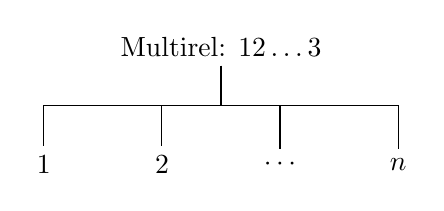
\begin{tikzpicture}
  \node {Multirel: $\rels1 \rels2 \ldots \rels3$}
    [edge from parent fork down]
    child {node {$\ex 1$}}
    child {node {$\ex 2$}}
    child {node {$\cdots$}}
    child {node {$\ex n$}}
    ;
\end{tikzpicture}


\subsection{Operator}

\textcolor{red}{The following might be rubbish\ldots}

The general operator rules are as follows:

\AXC{$A + B$}\RL{$infixop_1$}\UIC{+ A B}\DisplayProof\qquad 
\AXC{$\Phi + A$}\RL{$infixop_2$ with $\Phi\equiv + A_1\ldots A_n$}\UIC{$+ A_1 \ldots A_n A$}\DisplayProof 


\section{Schema}
\label{sec:schema}

A simple schema, ignoring attributes for the time being.

\begin{lstlisting}
<?xml version="1.0" encoding="utf-16"?>
<xsd:schema attributeFormDefault="unqualified" elementFormDefault="qualified" version="1.0" xmlns:xsd="http://www.w3.org/2001/XMLSchema">
  <xsd:element name="relseq" type="relseqType" />
  <xsd:complexType name="relseqType">
    <xsd:sequence>
      <xsd:element name="content" type="contentType" />
      <xsd:element name="children" type="childrenType" />
    </xsd:sequence>
  </xsd:complexType>
  <xsd:complexType name="childrenType">
    <xsd:sequence>
      <xsd:element maxOccurs="unbounded" name="infixop" type="infixopType" />
    </xsd:sequence>
  </xsd:complexType>
  <xsd:complexType name="infixopType">
    <xsd:sequence>
      <xsd:element name="content" type="contentType" />
      <xsd:element name="children" type="childrenType" />
    </xsd:sequence>
  </xsd:complexType>
  <xsd:complexType name="childrenType">
    <xsd:sequence>
      <xsd:element name="infixop" type="infixopType" />
      <xsd:element maxOccurs="unbounded" name="identifier" type="xsd:string" />
    </xsd:sequence>
  </xsd:complexType>
  <xsd:complexType name="infixopType">
    <xsd:sequence>
      <xsd:element name="content" type="contentType" />
      <xsd:element name="children" type="childrenType" />
    </xsd:sequence>
  </xsd:complexType>
  <xsd:complexType name="childrenType">
    <xsd:sequence>
      <xsd:element maxOccurs="unbounded" name="identifier" type="xsd:string" />
    </xsd:sequence>
  </xsd:complexType>
  <xsd:complexType name="contentType">
    <xsd:sequence>
      <xsd:element maxOccurs="unbounded" name="operator" type="xsd:string" />
    </xsd:sequence>
  </xsd:complexType>
</xsd:schema>
\end{lstlisting}



\section{Examples}
\label{sec:examples}


\subsection{Operators}
\label{sec:operators}

\subsubsection{Trivial}
\label{sec:trivial-ops}


\begin{lstlisting}
  <mi>a</mi>
  <mo>+</mo>
  <mi>b</mi>
  <mo>+</mo>
  <mi>c</mi>
\end{lstlisting}
\begin{lstlisting}
<infixop>+
  <content>
    <operator>+</operator>
    <operator>+</operator>
  </content>
  <children>
    <identifier>a</identifier>
    <identifier>b</identifier>
    <identifier>c</identifier>
  </children>
</infixop>
\end{lstlisting}



Simple Schema:
\begin{lstlisting}
<?xml version="1.0" encoding="utf-16"?>
<xsd:schema attributeFormDefault="unqualified" elementFormDefault="qualified" version="1.0" xmlns:xsd="http://www.w3.org/2001/XMLSchema">
  <xsd:element name="infixop" type="infixopType" />
  <xsd:complexType name="infixopType">
    <xsd:sequence>
      <xsd:element name="content" type="contentType" />
      <xsd:element name="children" type="childrenType" />
    </xsd:sequence>
  </xsd:complexType>
  <xsd:complexType name="childrenType">
    <xsd:sequence>
      <xsd:element maxOccurs="unbounded" name="identifier" type="xsd:string" />
    </xsd:sequence>
  </xsd:complexType>
  <xsd:complexType name="contentType">
    <xsd:sequence>
      <xsd:element maxOccurs="unbounded" name="operator" type="xsd:string" />
    </xsd:sequence>
  </xsd:complexType>
</xsd:schema>
\end{lstlisting}

\subsubsection{Combined}
\label{sec:combined-ops}


\begin{lstlisting}
  <mi>a</mi>
  <mo>+</mo>
  <mi>b</mi>
  <mo>+</mo>
  <mi>c</mi>
  <mo>-</mo>
  <mi>d</mi>
  <mo>-</mo>
  <mi>e</mi>
\end{lstlisting}
\begin{lstlisting}
<infixop>-
<content><operator>-</operator><operator>-</operator></content>
<children>
  <infixop>+
  <content><operator>+</operator><operator>+</operator></content>
  <children>
    <identifier>a</identifier>
    <identifier>b</identifier>
    <identifier>c</identifier>
  </children>
  </infixop>
  <identifier>d</identifier>
  <identifier>e</identifier>
</children>
</infixop>
\end{lstlisting}

Simple Schema:
\begin{lstlisting}
<?xml version="1.0" encoding="utf-16"?>
<xsd:schema attributeFormDefault="unqualified" elementFormDefault="qualified" version="1.0" xmlns:xsd="http://www.w3.org/2001/XMLSchema">
  <xsd:element name="infixop" type="infixopType" />
  <xsd:complexType name="infixopType">
    <xsd:sequence>
      <xsd:element name="content" type="contentType" />
      <xsd:element name="children" type="childrenType" />
    </xsd:sequence>
  </xsd:complexType>
  <xsd:complexType name="childrenType">
    <xsd:sequence>
      <xsd:element name="infixop" type="infixopType" />
      <xsd:element maxOccurs="unbounded" name="identifier" type="xsd:string" />
    </xsd:sequence>
  </xsd:complexType>
  <xsd:complexType name="contentType">
    <xsd:sequence>
      <xsd:element maxOccurs="unbounded" name="operator" type="xsd:string" />
    </xsd:sequence>
  </xsd:complexType>
</xsd:schema>
\end{lstlisting}



\subsection{Relations}
\label{sec:relations}

\begin{lstlisting}
  <mi>a</mi>
  <mo>=</mo>
  <mi>b</mi>
  <mo>=</mo>
  <mi>c</mi>
\end{lstlisting}

\begin{lstlisting}
<relseq>=
<content>
  <relation>=</relation>
  <relation>=</relation>
</content>
<children>
  <identifier>a</identifier>
  <identifier>b</identifier>
  <identifier>c</identifier>
</children>
</relseq>
\end{lstlisting}

\subsection{Mixed Operators and Relation}
\label{sec:operators-relations}

\begin{lstlisting}
  <mi>a</mi>
  <mo>+</mo>
  <mi>b</mi>
  <mo>+</mo>
  <mi>c</mi>
  <mo>-</mo>
  <mi>d</mi>
  <mo>-</mo>
  <mi>e</mi>
  <mo>=</mo>
  <mi>a</mi>
  <mo>-</mo>
  <mi>d</mi>
  <mo>+</mo>
  <mi>b</mi>
  <mo>+</mo>
  <mi>c</mi>
  <mo>-</mo>
  <mi>e</mi>
  <mo>=</mo>
  <mi>a</mi>
  <mo>+</mo>
  <mi>b</mi>
  <mo>-</mo>
  <mi>d</mi>
  <mo>-</mo>
  <mi>e</mi>
  <mo>+</mo>
  <mi>c</mi>
\end{lstlisting}

\pagebreak
\scriptsize
\begin{lstlisting}
  <relseq>
    =
    <content>
      <relation>=</relation>
      <relation>=</relation>
    </content>
    <children>
      <infixop>
        -
        <content>
          <operator>-</operator>
          <operator>-</operator>
        </content>
        <children>
          <infixop>
            +
            <content>
              <operator>+</operator>
              <operator>+</operator>
            </content>
            <children>
              <identifier>a</identifier>
              <identifier>b</identifier>
              <identifier>c</identifier>
            </children>
          </infixop>
          <identifier>d</identifier>
          <identifier>e</identifier>
        </children>
      </infixop>
      <infixop>
        -
        <content>
          <operator>-</operator>
        </content>
        <children>
          <infixop>
            +
            <content>
              <operator>+</operator>
              <operator>+</operator>
            </content>
            <children>
              <infixop>
                -
                <content>
                  <operator>-</operator>
                </content>
                <children>
                  <identifier>a</identifier>
                  <identifier>d</identifier>
                </children>
              </infixop>
              <identifier>b</identifier>
              <identifier>c</identifier>
            </children>
          </infixop>
          <identifier>e</identifier>
        </children>
      </infixop>
      <infixop>
        +
        <content>
          <operator>+</operator>
        </content>
        <children>
          <infixop>
            -
            <content>
              <operator>-</operator>
              <operator>-</operator>
            </content>
            <children>
              <infixop>
                +
                <content>
                  <operator>+</operator>
                </content>
                <children>
                  <identifier>a</identifier>
                  <identifier>b</identifier>
                </children>
              </infixop>
              <identifier>d</identifier>
              <identifier>e</identifier>
            </children>
          </infixop>
          <identifier>c</identifier>
        </children>
      </infixop>
    </children>
  </relseq>
\end{lstlisting}

\section{Examples}

\begin{lstlisting}
<math>
  <mi>5</mi>
  <mo>=</mo>
  <mi>3</mi>
  <mo>+</mo>
  <mi>2</mi>
</math>

<stree>
  <relseq role="equality" id="6">
    =
    <content>
      <relation role="equality" id="1">=</relation>
    </content>
    <children>
      <number role="integer" font="italic" id="0">5</number>
      <infixop role="addition" id="5">
        +
        <content>
          <operator role="addition" id="3">+</operator>
        </content>
        <children>
          <number role="integer" font="italic" id="2">3</number>
          <number role="integer" font="italic" id="4">2</number>
        </children>
      </infixop>
    </children>
  </relseq>
</stree>

<math>
  <mrow semantic-type="relseq" semantic-role="equality" id="6" semantic-content="1" semantic-children="0,5">
    <mi semantic-type="number" semantic-role="integer" id="0" semantic-parent="0">5</mi>
    <mo semantic-type="relation" semantic-role="equality" id="1" semantic-operator="=" semantic-parent="1">=</mo>
    <mrow semantic-type="infixop" semantic-role="addition" id="5" semantic-content="3" semantic-children="2,4" semantic-parent="5">
      <mi semantic-type="number" semantic-role="integer" id="2" semantic-parent="2">3</mi>
      <mo semantic-type="operator" semantic-role="addition" id="3" semantic-operator="+" semantic-parent="3">+</mo>
      <mi semantic-type="number" semantic-role="integer" id="4" semantic-parent="4">2</mi>
    </mrow>
  </mrow>
</math>
\end{lstlisting}

\end{document}


%%% Local Variables:
%%% mode: latex
%%% TeX-master: t
%%% End:
